\section{Evaluasi Model}

Model dilatih sesuai dengan konfigurasi yang telah disebutkan pada subbab \ref{sec:pelatihan-model} dan dilatih pada lingkungan eksperimen yang telah disebutkan pada subbab \ref{sec:lingkungan-eksperimen}. Eksperimen dilakukan pada setiap tugas evaluasi yaitu \nlptask dengan setiap tugas evaluasi dilatih dengan \textit{fine-tuning}, \methodPEFT. Hasil evaluasi dilakukan pada 5-\textit{fold} dengan setiap evaluasi terdapat nilai rata-rata, minimum, dan maksimum dari \textit{fold} tersebut.

\begin{table}[h]
    \centering
    \caption{Parameter model IndoBERT}
    \label{table:param-indobert}
    \begin{tabular}{|l|l|c|}
        \hline \rowcolor{black!10}
        \multicolumn{1}{|c|}{\textbf{Metode}} & \multicolumn{1}{|c|}{\textbf{Parameter}} & \textbf{\%Parameter} \\ \hline
        \textit{Fine-tuning} & 109.967.616 &  100 \\ \hline
        LoRA-r8 & 294.912 & 0,268 \\ \hline
        LoRA-r16 & 589.824 & 0,536 \\ \hline
        Prefix Tuning-pt10 & 9.857.024 & 8,964 \\ \hline
        Prefix Tuning-pt20 & 9.864.704 & 8,971 \\ \hline
        Prefix Tuning-pt30 & 9.872.384 & 8,978 \\ \hline
        Bottleneck Adapter & 894.528 & 0,893 \\ \hline
        UniPELT & 11.083.376 & 10,079 \\ \hline
    \end{tabular}
\end{table}

\begin{table}[h]
    \centering
    \caption{Parameter model IndoT5}
    \label{table:param-indot5}
    \begin{tabular}{|l|l|c|}
        \hline \rowcolor{black!10}
        \multicolumn{1}{|c|}{\textbf{Metode}} & \multicolumn{1}{|c|}{\textbf{Parameter}} & \textbf{\%Parameter} \\ \hline
        \textit{Fine-tuning} & 222.903.552 &  100 \\ \hline
        LoRA-r8 & 884.736 & 0,397 \\ \hline
        LoRA-r16 & 1.769.472 & 0,794 \\ \hline
        Prefix Tuning-pt10 & 29.571.072 & 13,266 \\ \hline
        Prefix Tuning-pt20 & 29.594.112 & 13,277 \\ \hline
        Prefix Tuning-pt30 & 29.617.152 & 13,287 \\ \hline
        Bottleneck Adapter & 1.789.056 & 0,803 \\ \hline
        UniPELT & 32.346.372 & 14,511 \\ \hline
    \end{tabular}
\end{table}

\subsection{Hasil Evaluasi NER}

\begin{figure}[h]
    \centering
    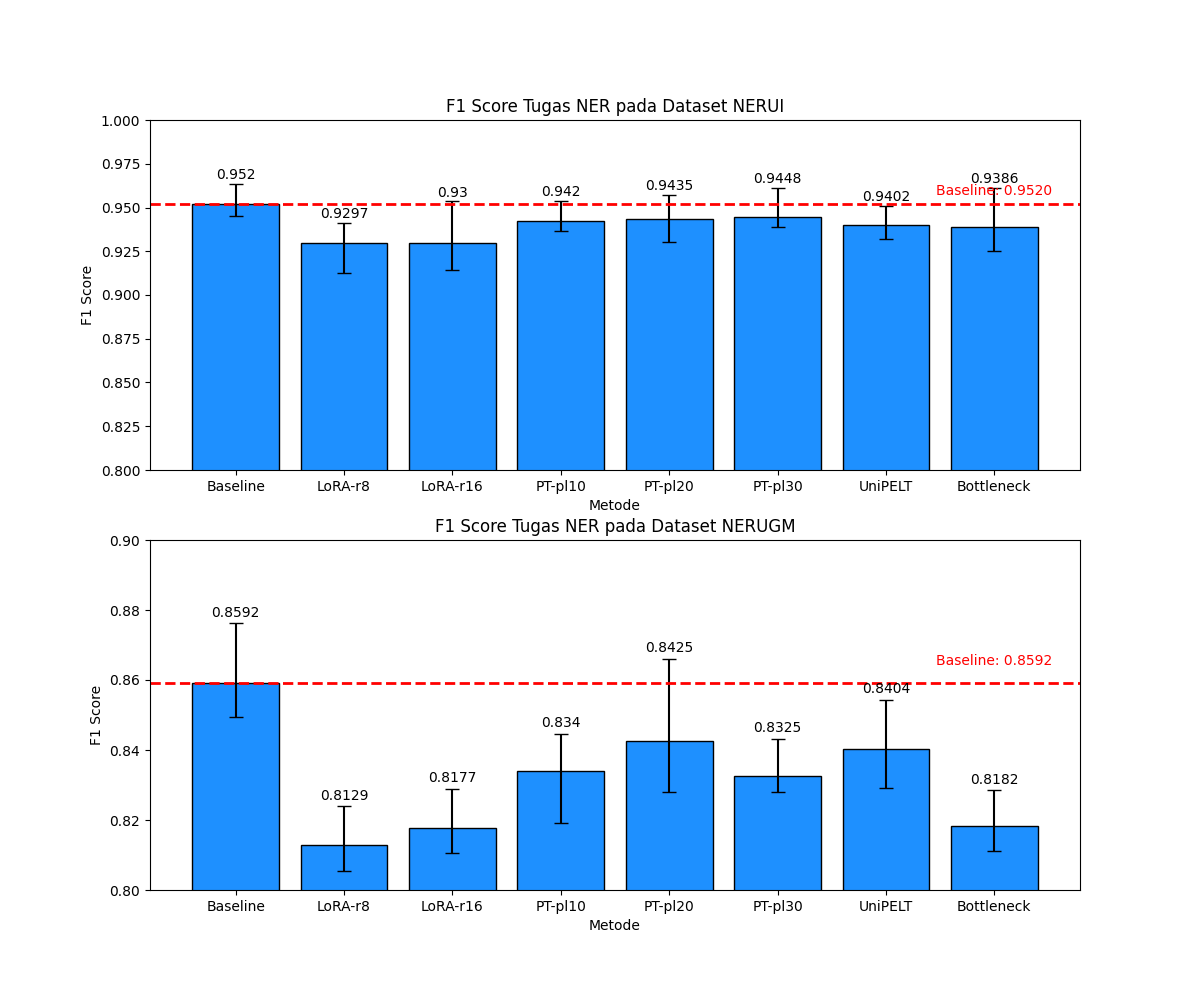
\includegraphics[width=\textwidth]{chapter-4/ner_eval_f1.png}
    \caption{\textit{F1 Score} Hasil Evaluasi NER}
    \label{fig:f1-ner}
\end{figure}

\begin{table}[h]
    \centering
    \caption{Waktu pelatihan tugas NER pada \textit{dataset} NERUI}
    \label{table:runtime-nerui}
    \begin{tabular}{|l|l|c|}
        \hline \rowcolor{black!10}
        \multicolumn{1}{|c|}{\textbf{Metode}} & \multicolumn{1}{|c|}{\textbf{Waktu(s)}} & \textbf{\%Peningkatan} \\ \hline
        \textit{Fine-tuning} & 923,2 & -  \\ \hline
        LoRA-r8 & 543,6 & 41,12 \\ \hline
        LoRA-r16 & 532,2 & 42,35 \\ \hline
        Prefix Tuning-pt10 & 552,6 & 40,14 \\ \hline
        Prefix Tuning-pt20 & 567,6 & 38,52 \\ \hline
        Prefix Tuning-pt30 & 612,5 & 33,65 \\ \hline
        Bottleneck Adapter & 581,8 & 36,98 \\ \hline
        UniPELT & 946 & -2.47 \\ \hline
    \end{tabular}
\end{table}

\begin{table}[h]
    \centering
    \caption{Waktu pelatihan tugas NER pada \textit{dataset} NERUGM}
    \label{table:runtime-nerugm}
    \begin{tabular}{|l|l|c|}
        \hline \rowcolor{black!10}
        \multicolumn{1}{|c|}{\textbf{Metode}} & \multicolumn{1}{|c|}{\textbf{Waktu(s)}} & \textbf{\%Peningkatan} \\ \hline
        \textit{Fine-tuning} & 1.155,6 & -  \\ \hline
        LoRA-r8 & 597,4 & 48,3 \\ \hline
        LoRA-r16 & 605,4 & 47,61 \\ \hline
        Prefix Tuning-pt10 & 640,4 & 44,58 \\ \hline
        Prefix Tuning-pt20 & 645,8 & 44,12 \\ \hline
        Prefix Tuning-pt30 & 646,8 & 44,03\\ \hline
        Bottleneck Adapter & 632 & 45,31 \\ \hline
        UniPELT & 1011 & -12,51 \\ \hline
    \end{tabular}
\end{table}

\subsection{Hasil Evaluasi \textit{Sentiment Analysis}}

\begin{figure}[h]
    \centering
    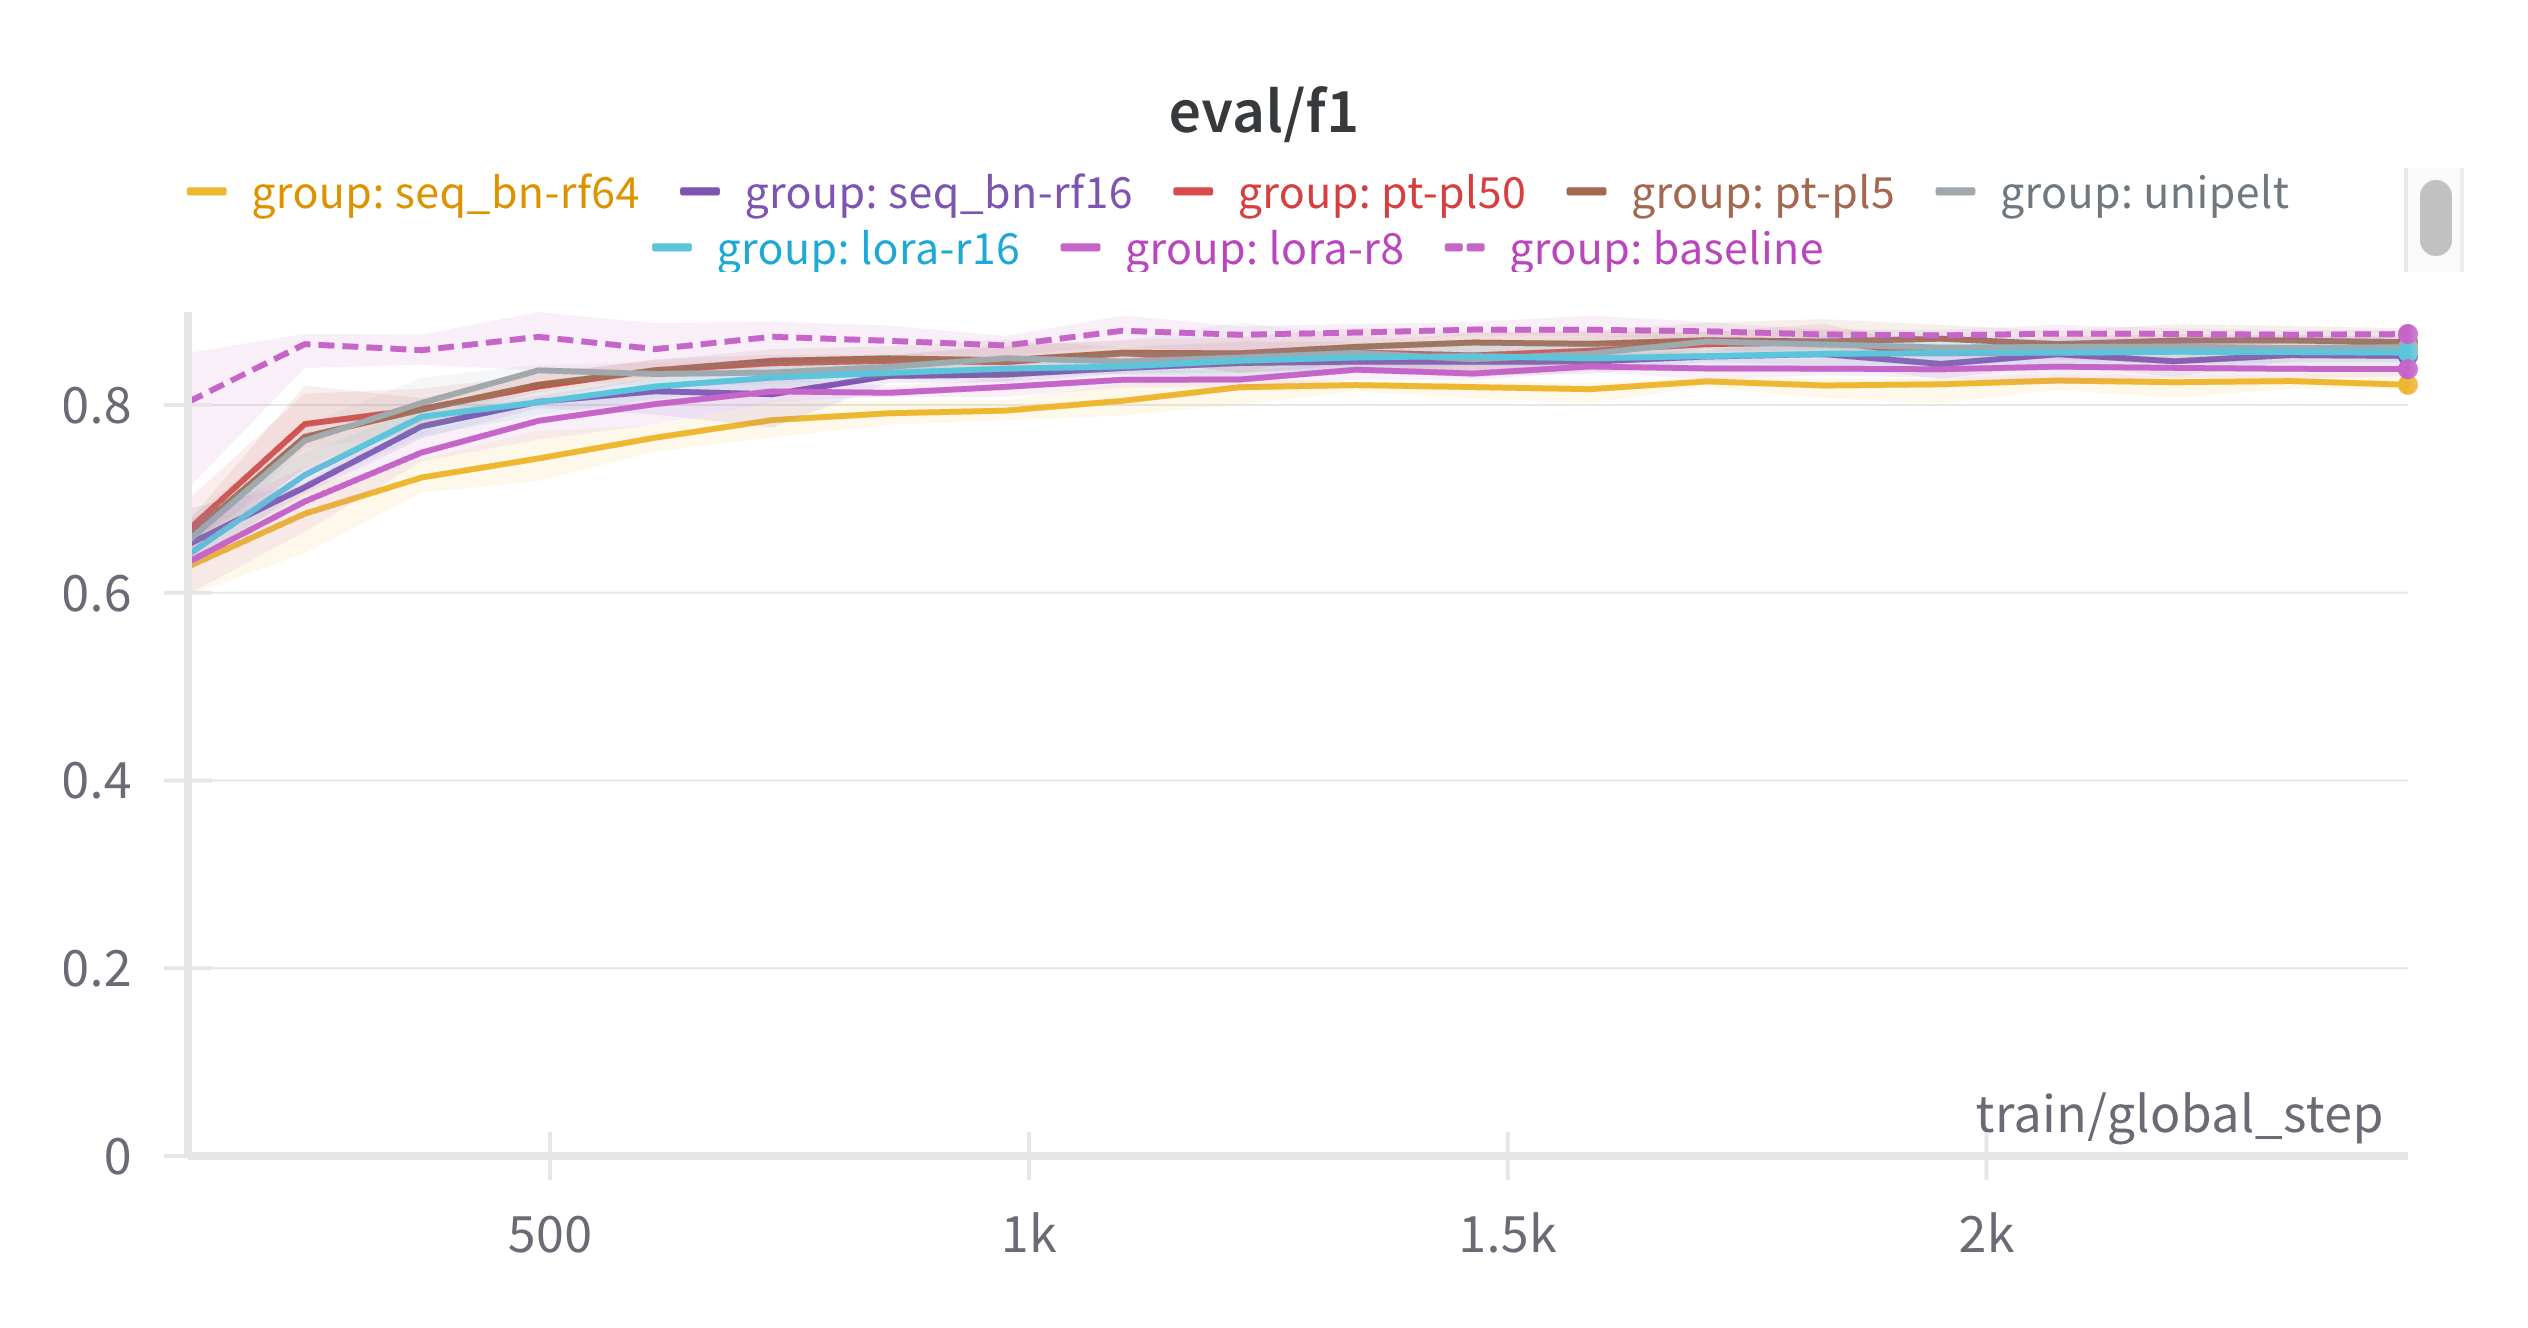
\includegraphics[width=\textwidth]{chapter-4/sentiment_eval_f1.png}
    \caption{\textit{F1 Score} Hasil Evaluasi \textit{Sentiment Analysis}}
    \label{fig:sentiment-ner}
\end{figure}

\begin{table}[h]
    \centering
    \caption{Waktu pelatihan tugas \textit{sentiment analysis}}
    \label{table:runtime-sentiment}
    \begin{tabular}{|l|l|c|}
        \hline \rowcolor{black!10}
        \multicolumn{1}{|c|}{\textbf{Metode}} & \multicolumn{1}{|c|}{\textbf{Waktu(s)}} & \textbf{\%Peningkatan} \\ \hline
        \textit{Fine-tuning} & 905,6 & -  \\ \hline
        LoRA-r8 & 652,4 & 27,96 \\ \hline
        LoRA-r16 & 652 & 28 \\ \hline
        Prefix Tuning-pt10 & 646,4 & 28,62 \\ \hline
        Prefix Tuning-pt20 & 652,6 & 27,94 \\ \hline
        Prefix Tuning-pt30 & 661,4 & 26,97 \\ \hline
        Bottleneck Adapter & 641,8 & 29,13 \\ \hline
        UniPELT & 771,6 & 14,8 \\ \hline
    \end{tabular}
\end{table}

\subsection{Hasil Evaluasi \textit{Summarization}}

\begin{figure}[h]
    \centering
    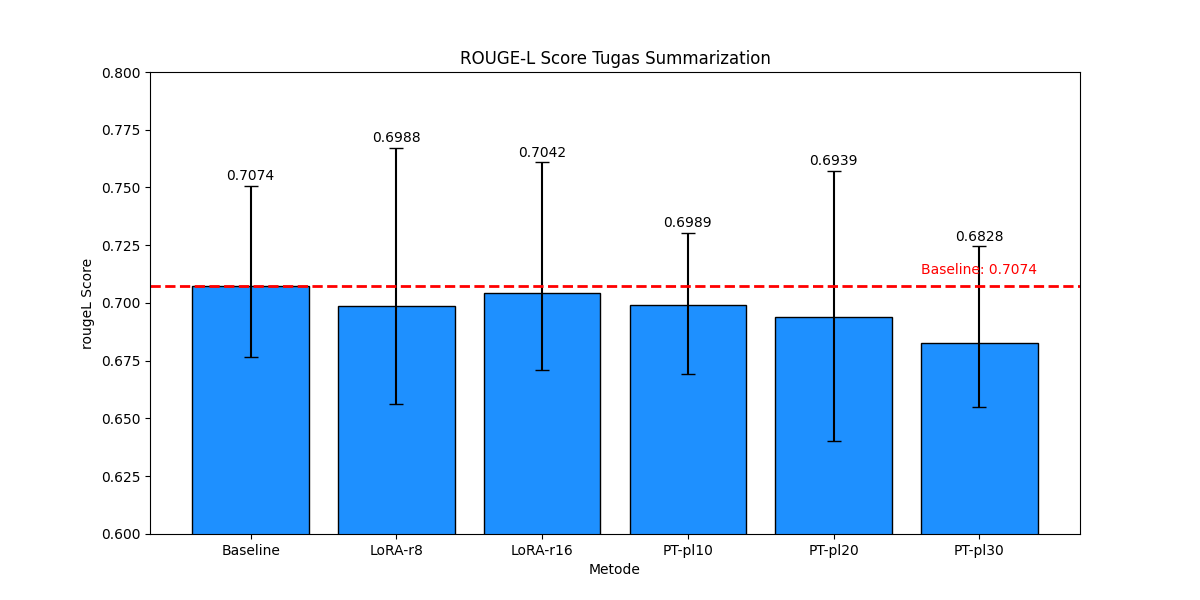
\includegraphics[width=\textwidth]{chapter-4/summarization_eval_rougeL.png}
    \caption{ROUGE-L \textit{Score} Hasil Evaluasi \textit{Summarization}}
    \label{fig:summarization-rouge-l}
\end{figure}

\begin{table}[h]
    \centering
    \caption{Waktu pelatihan tugas \textit{summarization}}
    \label{table:runtime-summarization}
    \begin{tabular}{|l|l|c|}
        \hline \rowcolor{black!10}
        \multicolumn{1}{|c|}{\textbf{Metode}} & \multicolumn{1}{|c|}{\textbf{Waktu(s)}} & \textbf{\%Peningkatan} \\ \hline
        \textit{Fine-tuning} & 7189,6 & -  \\ \hline
        LoRA-r8 & 7500,8 & -4,33 \\ \hline
        LoRA-r16 & 6970,6 & 3,05 \\ \hline
        Prefix Tuning-pt10 & 8296,6 & -15,4 \\ \hline
        Prefix Tuning-pt20 & 8298,6 & -15,43 \\ \hline
        Prefix Tuning-pt30 & 8484,4 & -18,01 \\ \hline
    \end{tabular}
\end{table}
